\section{Vortex Generator}

It is desirable to enhance understanding of 
trailing axial vortices generated by aircraft wingtips.
While naturally occurring axial vortices occur in unpredictable and non-uniform 
environments, this experimental investigation required a repeatable axial 
vortex.  Small-scale aircraft axial wake vortices can be generated in an 
enclosed wind tunnel environment with a single wingtip, but the downwash 
behavior resulting from a lift-generating wingtip vortex causes the rotational 
axis to curve and become distorted by the walls of the wind tunnel and
test section. A bi-wing vortex generator, as pictured in Figures 
\ref{fig:vortex_gen} and \ref{fig:vortex_design}, was designed and constructed 
by undergraduate student researchers to generate a vortex with two opposing 
wings, producing a single vortex, absent any downwash effects \cite{davis2012}. 
The vortex generator employed two symmetric NACA-0012
airfoils with chord lengths of 101.6$mm$, manufactured from foam casts. Both 
airfoils were attached 
to a 25.4$mm$ diameter cylindrical center body with hemispherical forward and 
aft end caps. While the vortex generator could have allowed angles-of-attack 
adjustments, the precision with which the adjustments could be made was 
considered to be inadequate for producing repeatable results, so the wings were 
locked at angles-of-attack of $\pm$8 degrees.

\vspace{32pt}
\begin{figure}[H]
\centering
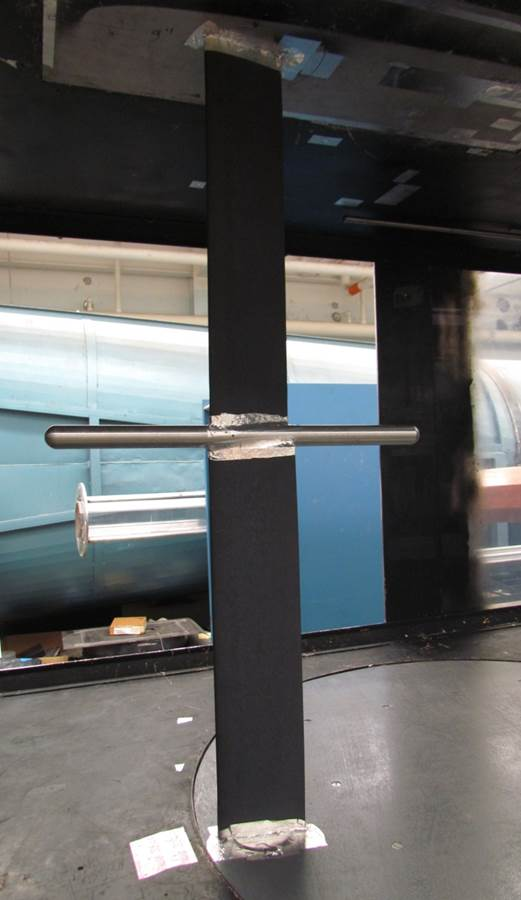
\includegraphics[width=4in]{figs/setup/vortex_generator/picture}
\caption{Picture of the vortex generator set up in the ODU LSWT.}
\label{fig:vortex_gen}
\end{figure}

\begin{figure}[H]
\centering
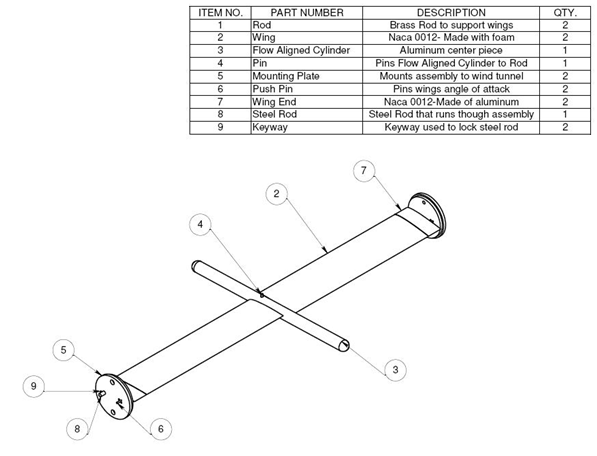
\includegraphics[width=5.75in]{figs/setup/vortex_generator/design}
\caption{CAD design of the vortex generator used in this study.}
\label{fig:vortex_design}
\end{figure}

